\subsection{Segundo Prototipo}
El segundo prototipo modela el comportamiento del primer nivel del juego (ver 
apartado \ref{Niveles}). 

\subsubsection{Creación de Sprites}
Para este prototipo se crearon todos los sprites a utilizar, salvo por los botones 
de la Interfaz de usuario, ya que estos se conservaron del prototipo anterior. En 
total se crearon:
\begin{itemize}
	\item Tres imágenes de fondo.
	\item Tres iconos.
	\item Diez imágenes para la animación de Malinalli.
	\item Seis imágenes para la animación de Xólotl en su forma xoloitzcuintle.
	\item Seis imágenes para la animación de Xólotl en su forma humano.
	\item Una imagen para Quetzalcóatl.
	\item Cinco imágenes para los ciudadanos
	\item Cuatro imágenes para el suelo.
	\item Cuatro imágenes para los objetos de fondo de la ciudad.
	\item Dos imágenes para los objetos de fondo de la jungla.
	\item Cinco imágenes para la animación del Jaguar.
\end{itemize}  
Consultar \ref{SpriteDic} para ver el resto de los sprites creados.

\subsubsection{Menú principal}
En este apartado se modificó la propuesta de diseño que se tenía en las interfaces 
(ver apartado \ref{TraReaInterfaces}). Tal como se puede ver en la figura 
\ref{figDisenioMenu}, la posición de los botones del prototipo varía con 
respecto a la del diseño. 
\\
\par
Al igual que en el prototipo uno, se configuraron los botones y el 
canvas para que adapten su tamaño si se modifica el tamaño de la 
pantalla.
\\
\par
Para la funcionalidad del menú principal se implementó la clase PrincipalMenuCtrl; 
sin embargo, no se implementaron todos sus métodos ni todos sus atributos. Siendo 
el botón Empezar partida, él unico con la funcionalidad parcialmente habilitada, 
ya que al ser oprimido por el jugador solo realiza la transición de la interfaz del 
menu principal a la primera mitad del nivel uno sin generar el archivo de datos 
de partida.
\\
\par

\begin{figure}
  \centering
   \subfigure[Propuesta de diseño para la interfaz del menú principal (Autoría propia).] {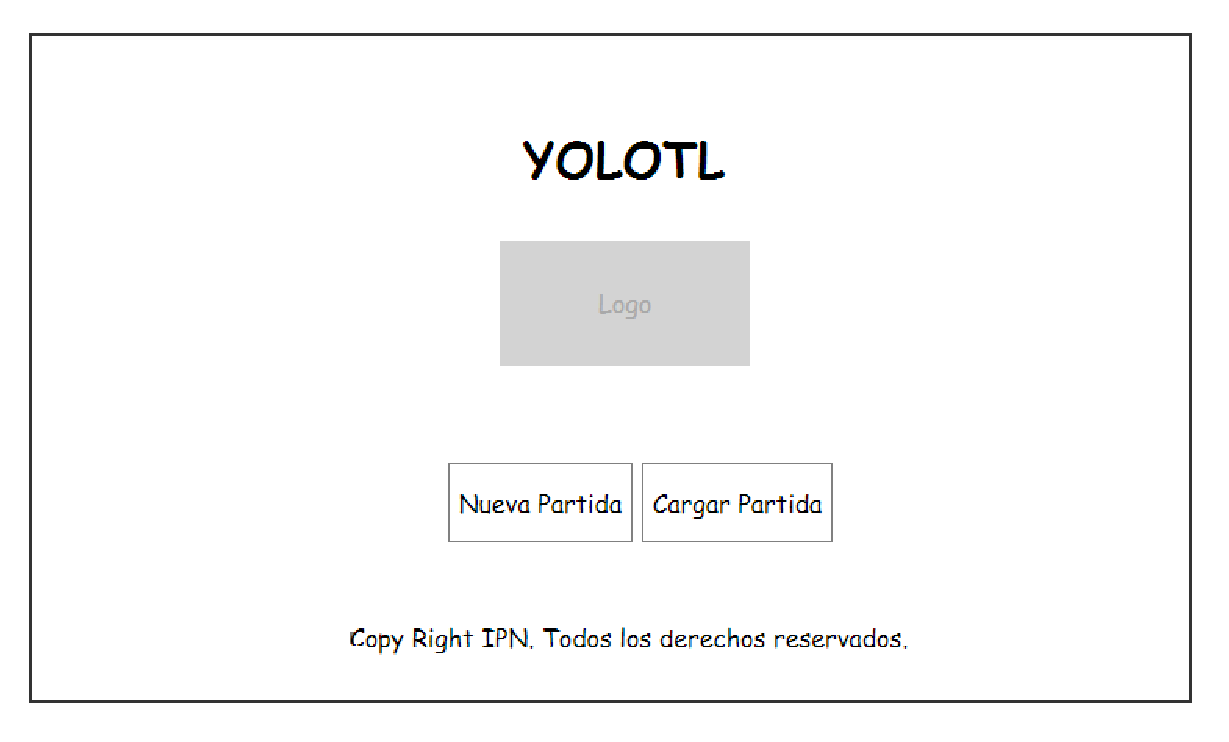
\includegraphics[width=0.4 \textwidth]{05TrabajoRealizado/03Unity/imagenes/interfaz01}}
   
 	\subfigure[Diseño final del menú principal (Autoría propia).] {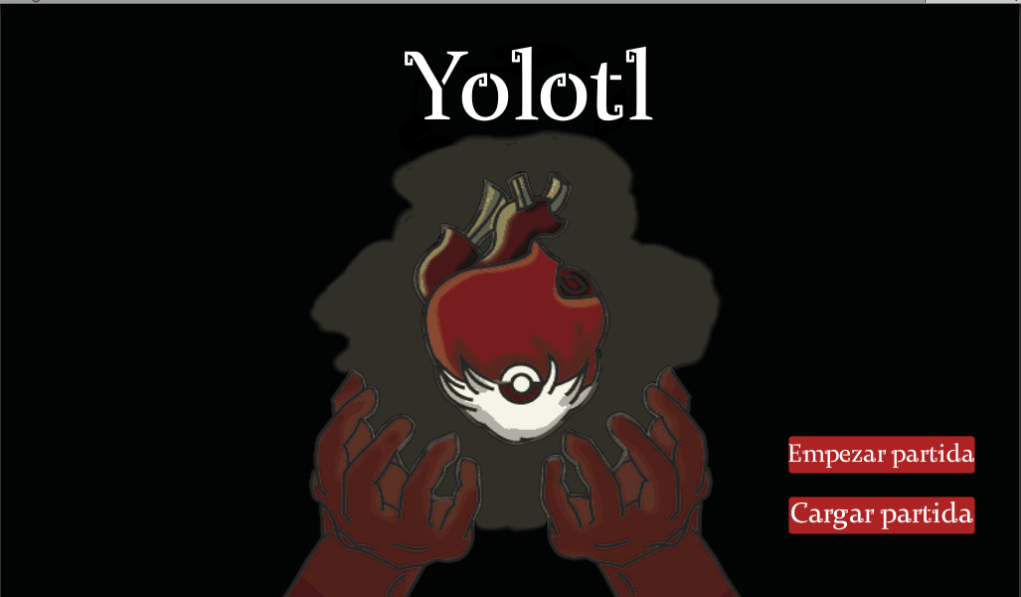
\includegraphics[width=0.4 \textwidth]{05TrabajoRealizado/03Unity/imagenes/menuPrincipalFinal}}
 	
  \caption{La implementación del menu principal varía la posición de los botones con respecto a la propuesta de diseño.}
  \label{figDisenioMenu}
\end{figure} 

\subsubsection{Implementación personaje jugable}
En cuanto a la implementación del personaje jugable, se trató de reutilizar la lógica 
del primer prototipo, con algunas diferencias. A continuación
se listan los cambios más significativos con respecto a la clase del prototipo anterior:
\begin{itemize}
	\item La clase \textit{Player} y la clase \textit{GroundCollisionCtrl} son las 
	encargadas de la funcionalidad del personaje jugable.
	\item La clase \textit{Player} deja de instanciar clases de tipo Controlador.
	\item El estado \textit{Idle} de la maquina de estados se renombra como
	 \textit{Normal} (ver Figura \ref{figMaqMalinalli}).
	 \item El sprite del personaje jugable corresponde con el diseño del personaje 
	 principal del juego propuesto en el documento de diseño (ver figura \ref{figAniMalinalli})
	 \item Se manejan atributos de tipo boolean como banderas de 
	 activación en los métodos que vinculan la clase \textit{Player} con la clase 
	 \textit{MobileUICtrl}.
\end{itemize}

\begin{figure}
  \centering
   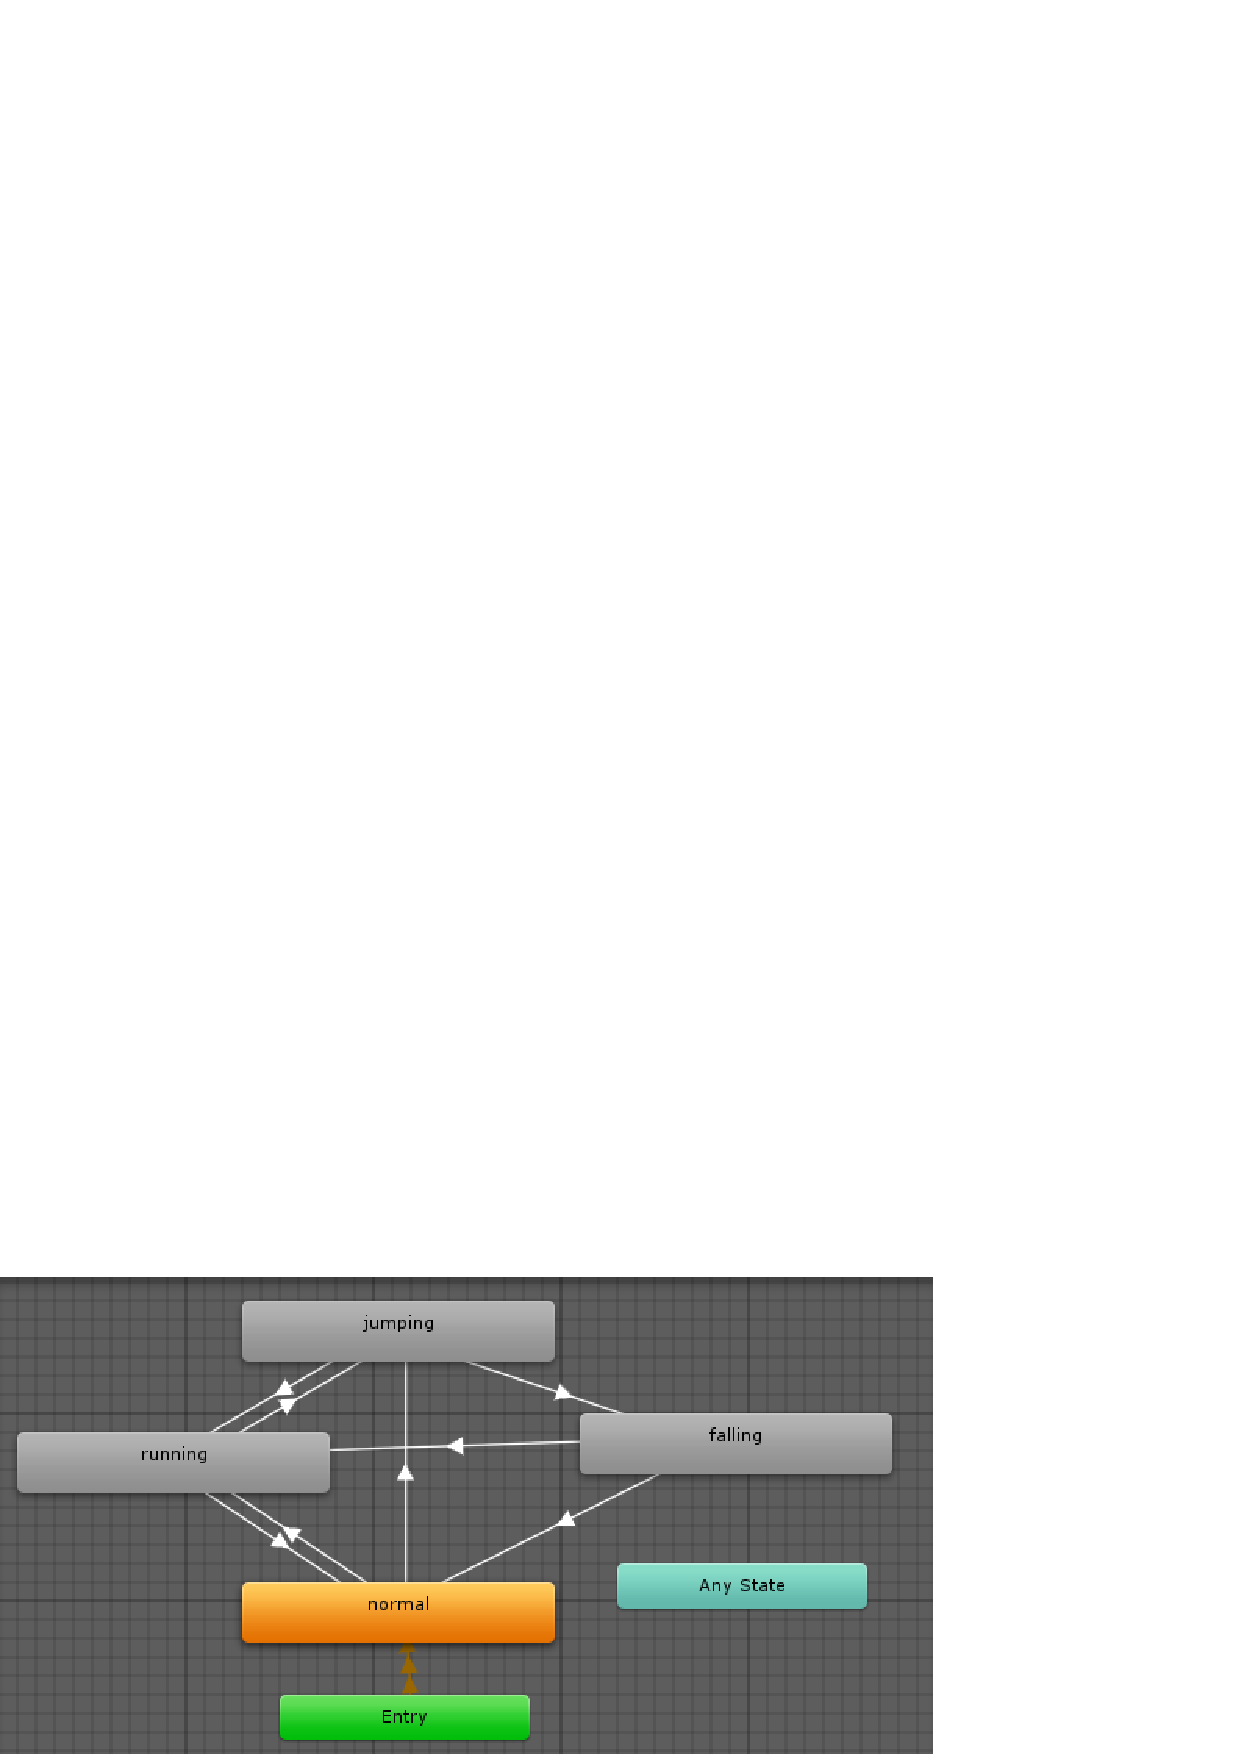
\includegraphics[width=0.4 \textwidth]{05TrabajoRealizado/03Unity/imagenes/03MaquinaEstadosMalinalli}
  \caption{Maquina de estados para la animación del personaje jugable Malinalli (Autoría propia)}
  \label{figMaqMalinalli}
\end{figure}

\begin{figure}
  \centering
   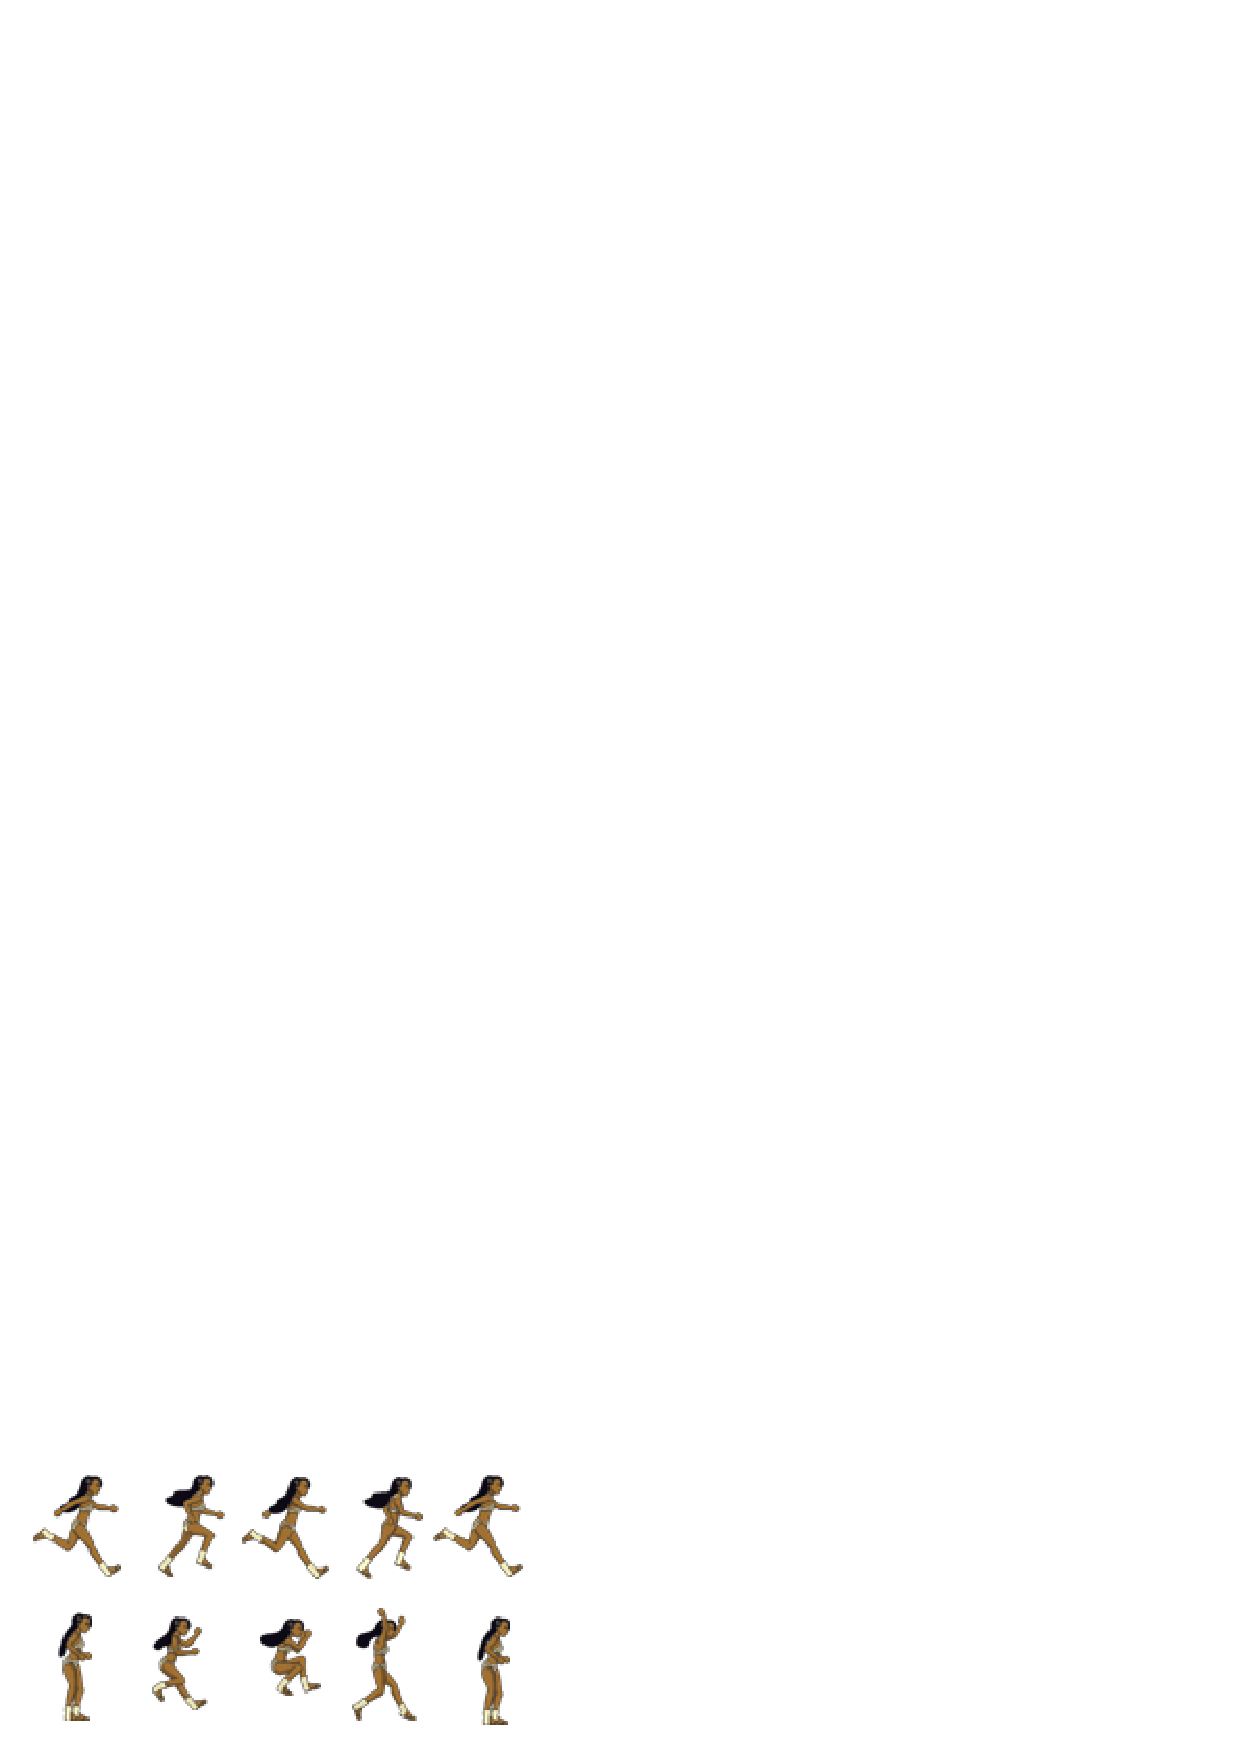
\includegraphics[width=0.4 \textwidth]{05TrabajoRealizado/03Unity/imagenes/bloquesanimacionMalinalli}
  \caption{Animacion de Run y Jump del personaje jugable Malinalli (Autoría propia)}
  \label{figAniMalinalli}
\end{figure}

\subsubsection{Interfaz gráfica del nivel}
Al igual que el prototipo anterior, la interfaz gráfica se compone de dos canvas: uno 
para los marcadores y otro para los botones que permiten al jugador controlar al personaje jugable (Ver figura \ref{figCanvasM}).
\\
\par
El canvas que contiene a los botones se mantinen si cambios referentes a su 
visualización; no obstante, los métodos de la clase Player que se activan con 
éstos varían. En este nivel el método FireGUI de la clase MobileUICtrl se 
remplaza por el método de GUIStartConversation de la clase TalkedCharacter; no 
obstante todas las clases referentes a la lectura y activación de dialogos no 
fueron implementadas por lo que el Botón de disparo se encuentra sin funcionalidad.
\\
\par
Por su parte el canvas que contiene los marcadores modifica su estructura visual (ver 
figuar \ref{figCanvasM}). Los corazones que indicaban la cantidad de vidas del 
prototipo anterior por una barra de vida y se agrega por primera vez la  
barra de cantidad Tonalli.   

\begin{figure}
  \centering
   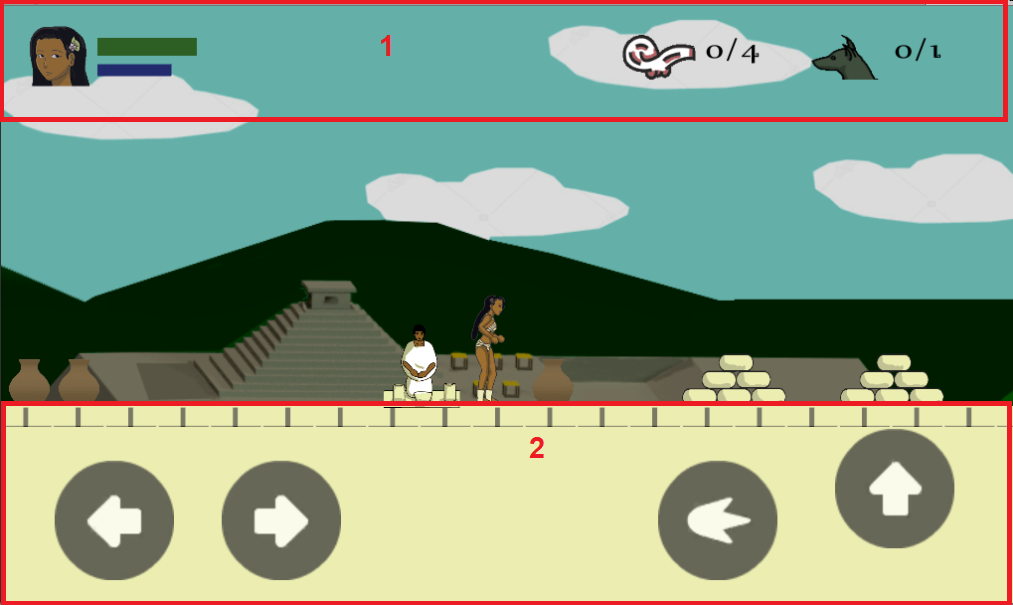
\includegraphics[width=0.4 \textwidth]{05TrabajoRealizado/03Unity/imagenes/03Interfaz}
  \caption{La interfaz gráfica se encuetra compuesta por dos canvas: 1. Contenedor de los marcadores. 2. Contenedor de los botones que permiten el control al personaje jugable (Autoría propia)}
  \label{figCanvasM}
\end{figure}

\subsubsection{Primer mitad del nivel uno}
Tomando la maqueta del primer nivel como base, se crearon los GameObjects 
correspondientes para construir la primera parte del primer nivel (ver \ref{Mac01}). 
 En esta primera mitad del prototipo no se alcanzó a crear la clase DialogueCtrl y todas sus clases ligadas por lo que se creó un GameObject vació, se le agregó el componente Box Collider2D, y se agrego una  de este modo se realiza la transición a la segunda mitad del primer nivel.
 
 \subsubsection{Segunda mitad del primer nivel}
 En esta segunda mitad se implementó la clase FollowedCharacter para la persecución 
 de Xólotl en su forma xoloitzcuintle. En Xólotl también fue necesario implementar 
 una maquina de estados para sus animación. Como se puede ver en la figura \ref{figAniXolo} la  maquina de estados de Xólotl esta compuesta de dos estados: .
 
 \begin{figure}
  \centering
   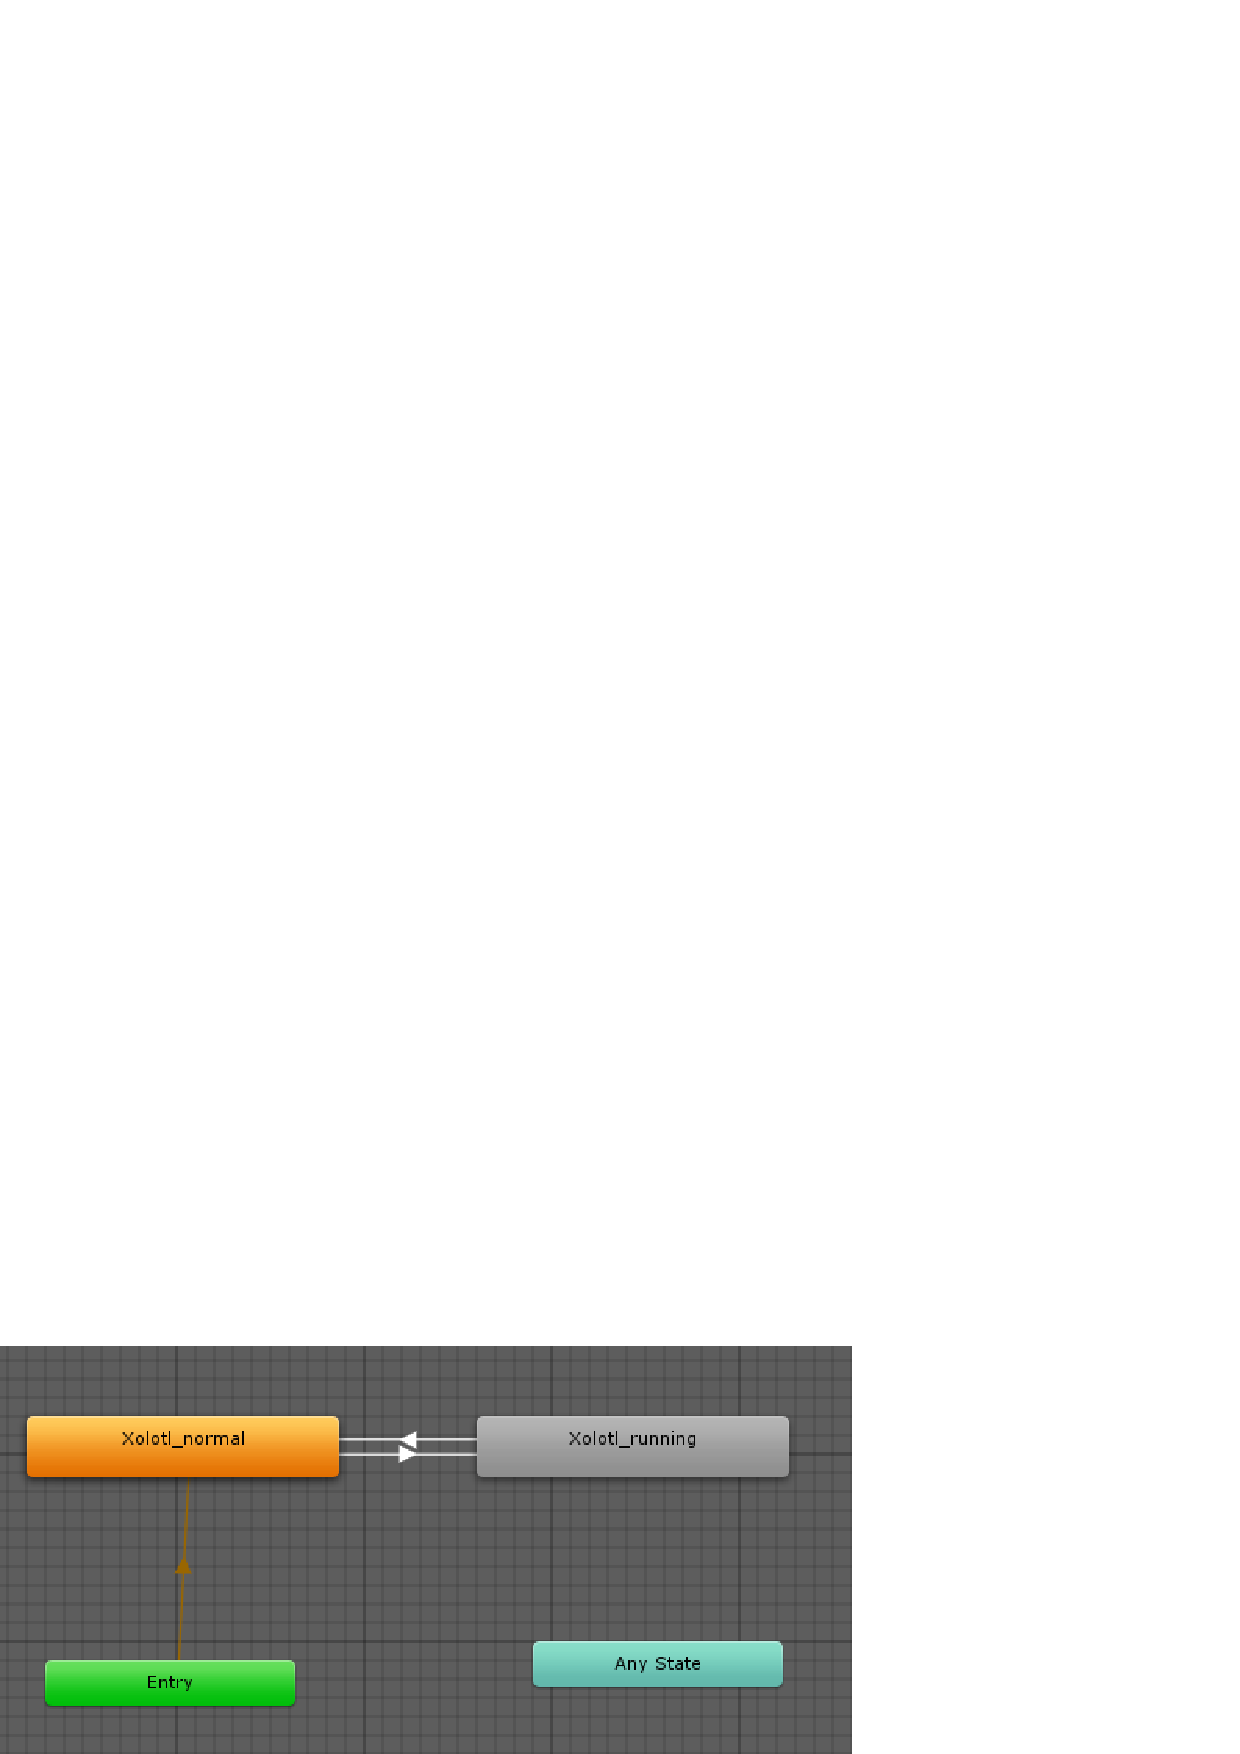
\includegraphics[width=0.4 \textwidth]{05TrabajoRealizado/03Unity/imagenes/03MaquinaEstadosXolotl}
  \caption{Maquina de estados de Xólotl forma xoloitzcuintle (Autoría propia)}
  \label{figAniXolo}
\end{figure}